Let's assume a BTS algorithm without propagation at all. In this case, to find out the constraints satisfaction we should try all the possible combinations
and test the assignments done. Basically we perform a \textbf{Depth-first search strategy} and whenever all the variables of a constraint are instantiated,
we check the validity of the constraint. \vspace{7pt}

It may seem quite stupid: first of all we do all the assignments and then we check if the constraint is satisfied or not. However, by this approach we can 
reach a final solution or prove the unsatisfiability of the problem. \vspace{7pt}

Instead, with propagation \textbf{before} the assignments we attempt to remove obvious useless values, or in other words all those values that do not 
have a \textbf{support}.
\begin{example}
    e.g. BTS example without propagation. \vspace{7pt}

    Starting from the below variables, domains and constraints: 
    $$
        \begin{gathered}
            D(X_1) = \{1, 2\}, D(X_2) = D(X_3) = \{1, 2, 3\} \\ 
            C_1 : X_1 \neq X_2, C_2 : X_2 < X_3
        \end{gathered}
    $$ 
    we can reach the final solution:
    $$ X_1 = 1, X_2 = 2, X_3 = 3 $$
    stating the following search tree. \vspace{3.5pt}
    \begin{center}
        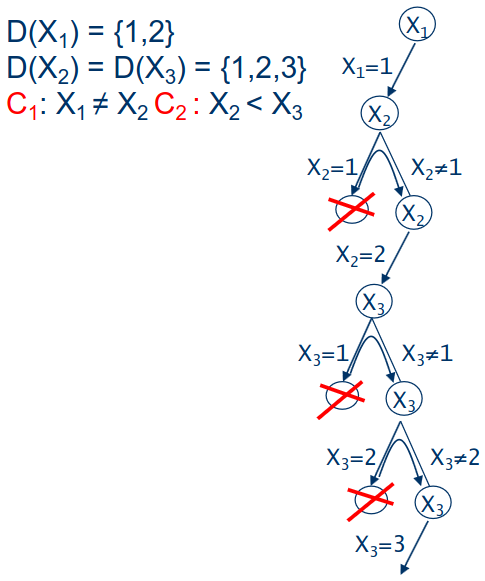
\includegraphics[width = 0.5\textwidth]{img/img17.png}
    \end{center} \vspace{3.5pt}
    This is a very stupid example: we are assigning values to variables without checking before the requirements of the constraints.
\end{example}